\documentclass[]{article}
\usepackage{multicol}
\usepackage[margin = 1.25in]{geometry}
\usepackage{graphicx}
\usepackage{mathtools}
\usepackage{caption}
\usepackage{lipsum}
\usepackage{algpseudocode}
\usepackage{fancyvrb}
\usepackage{amsfonts}
\usepackage{amsmath}
\newenvironment{Figure}
  {\par\medskip\noindent\minipage{\linewidth}}
  {\endminipage\par\medskip}

\linespread{2.0}
\setlength{\parskip}{1em}
%opening
\title{Modeling User Transition Behavior Among Networks With a Probabilistic Programming Approach}
\date{December 15, 2015}
\author{Shidan Xu}


\begin{document}
\maketitle

%\begin{abstract}
%
%\end{abstract}



\section{Abstract}

This paper describes a thesis project to be carried out at the MIT Advanced Networks Architecture (ANA) group. This project involves predicting a user's behavior in various networks. In particular, we are interested in how the user is likely to transition between networks. We plan to design various models to predict the user's behavior, and use various evaluation criteria to understand which model most vividly captures the user's behavior. As a learning experience for our team and me, we employ probabilistic programming (PP) techniques. PP is a way of programming that utilizes existing software packages that include encapsulated methods for the inference step of machine learning. By simplifying the implementation, it allows researchers to focus on models. This project has two main objectives. The first is to design several models to capture one or multiple aspects of a typical user, or a group of users' behavior in a network. The second is to evaluate each model to decide which model is more feasible, and which model is applicable under what situations. Together this project aims to give a better understanding of how network user transitions.

\section{Introduction}

This project relates to the FIND (Future Internet Design) initiative \cite{find}, which asks the question of what the requirements should be for a global network 15 years from now, and how we can build such a network if we are not constrained by the current Internet. The current Internet has made some design choices with assumptions. One particular assumption the Internet is making is that network mobility is similar to mobility in geography\cite{jacobson}. In reality we found that to be not necessarily true. A user could transition from a 4G network to Wi-Fi by walking a few meters in real world, but the IP addresses in network topology is likely to be not adjacent, even entirely different. In extreme cases, the nearest common ancestor of nodes in network topology can be on opposite coasts of the country. Such design is costly for the user to transition between networks. In designing a new network, one of the focal points is to decrease such inconsistency, as packets of information need to be rerouted.


The first step in creating an efficient network is to know the users. One of the actions we can evaluate is user transition. The bulk of this proposed work hence relates to evaluating and predicting how the user is likely to transition between networks, given his/her information. The workflow of this project is to 

\begin{itemize}
\item
Process Datasets
\item
Build a model
\item
Evaluate the model's performance
\item
Recurse steps 2 \& 3, with updated/new model.
\end{itemize}

We examine each step in the next sections.

\section{Datasets}

Multiple datasets exist for carrying out this research. We decided to first reproduce the Yang paper \cite{yang} results as a baseline. Hence we start out by exploring the UMass dataset. The UMass dataset contains user email activity in the form of IMAP logs for residents of University of Massachusetts at Amherst$^{(1)}$. The dataset includes user information such as the identity, the time of action, and action in terms of attaching to network, detaching from network, IP address, and the device used to log in. With this information, we can decide whether a transition happens from the logs. Brian Copeland, a UROP student of the group, parsed the original log entries into SQL entries that contain each individual session, or duration when the user is on a particular network. We can easily overlay the durations to decide occurrences of transition. The details of transition criteria can be found in Yang [3] paper.

\section{Modeling}
Given the dataset, we want to model how the user is likely to transition. In general, there are two categories of models we can use, generative vs. discriminative. A discriminative algorithm learns what criteria separate the classes given the dataset.  For instance, logistic regression is a discriminative algorithm. A generative model, focuses on each class, and creates a model for what the underlying process for each class is \cite{ng}. For x the features, y the output, discriminative models learn $Pr(y | x)$, whereas generative models learn $Pr(x | y)$. Therefore, generative model allows researchers to synthesize new dataset by understanding what the underlying distribution is. Since we are predicting user behavior, we lean towards using generative models. 


\begin{center}
    \begin{tabular}{| l | l | l | l |}
    \hline
     Transition Prob.& On 0 Networks & On 1 Network & On $>=1$ Networks\\ 
    \hline
    On 0 Networks CRF& 0.905 &0.088 & 0.007\\ 
    On 1 Network& 0.587 &0.352 & 0.061\\ 
    On $>=1$ Networks & 0.209 & 0.322 & 0.469\\
    \hline
    \end{tabular}
\captionof{table}{Preliminary empirical estimates of transition probabilities. Data acquired on a smaller training sample (1000 user days).}
\end{center}

For preliminary baseline, we reproduce the UMass three-state hidden Markov model. We model the user in three states: not on a network, on one network, on multiple networks. A 3 by 3-state transition matrix can be calculated directly from the dataset. We take measurements at the end of each 15-minute period. In table 1, we have the transition probability matrix calculated on a 1000 user days training sample. Given this transition probability matrix, we can generate estimations of what the user may behave in the future. We do not necessarily believe that such modeling optimally captures user behavior, but it serves as a baseline. 


The more complex version involves using more features. The original dataset includes information on type of phone, time of log, user action, ip address, etc. These are not enough features to describe a user's behavior. The idea here is twofold. 1. To acquire more information from the data we have. 2. To join the current dataset with more features that are available. An example of 1. is to acquire the geolocation of the IP addresses. An example of 2. is to join the dataset with weather of the day. For instance, when it snows, the user is more likely to stay indoors; the number of transitions may be fewer. 

We plan to learn the weights of these features through machine learning. First we separate the original dataset into training and validation datasets by time. Based on the training dataset, we build a model to extrapolate how the user will behave, and compare with the validation dataset. Machine learning is useful when humans have ambiguity in deciding which features are important. We rely on statistical analysis to help us distinguish the valuable features. This problem is exactly so, we have some ambiguous thoughts on which features can probably affect the user behavior, but we do not know how much they do.

The UMass dataset is rather simplistic with minimal useful information, and suffers from information loss, as some entries of device id are not available. We do not expect our results to be amazing using the machine learning approach as we have limited features. We have the option of extending the work to a broader, more complex dataset, if the legal process can proceed. 

\section{Evaluation}
The performance of a model needs to be assessed using some evaluation criteria. One evaluation criterion for the hidden Markov model can be the duration that we predicted the user to be on a particular network vs. actual duration. The HMM can predict a list of transition, from which we can study when exactly is the user on how many networks. Then, we can compare this time series data vs. the actual data, to see which period we are correct / not correct. Another type of evaluation can be whether we are correctly predicting the sequence of network transitions. This would be useful if the user follows a daily routine. Various evaluations explore various aspects of the models, and the models may beat each other under different evaluation metrics. The exact metric possibly needs more fine tuning.

For baseline, we evaluate the distribution of the number of transitions for all users on a daily basis as noted in Yang. We naively identify a transition as a change of state (on 0, on 1, or on 2 or more) from the end of the previous 15 minute period to the end of the current 15 minute period. We compute one distribution from the testing dataset, and another for the randomly generated dataset based on HMM runs. We make the simple assumption that all users behave similarly and the transition distributions are approximately normal. 

\begin{Figure}
 \centering
 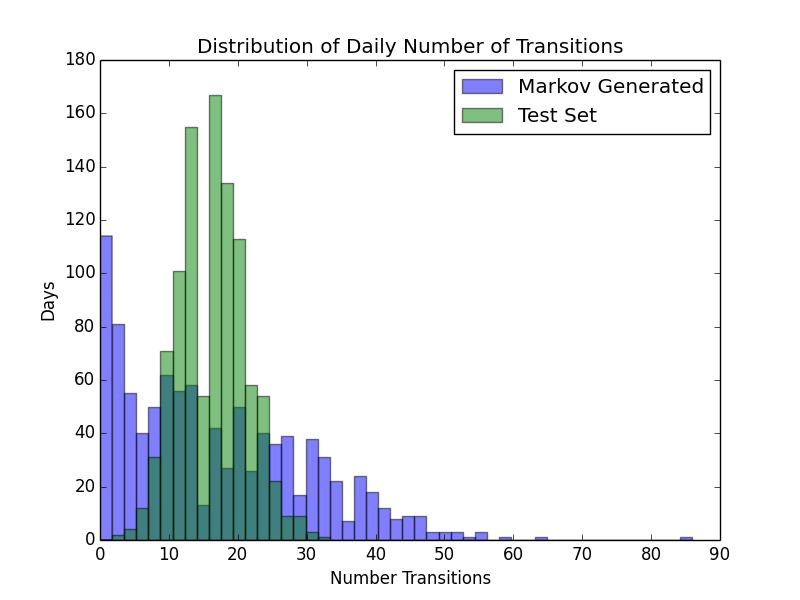
\includegraphics[height = 11cm, width =15cm]{figure_1.png}
 \captionof{figure}{The distribution of number of transitions from HMM and testing set. Sample size 1000 each.}
\end{Figure}

In figure 1, we illustrate the distribution of daily transitions for 1000 sample days generated by the HMM and 1000 days from the testing data. The testing data shows a more Gaussian distribution, whereas the HMM generated data shows a skewed tail. Despite the two datasets having similar transition probability matrices, the HMM failed to capture the normal distribution. Based on this very simple metric, we see that probability transition matrix alone does not capture the transition behavior.

This is a minimal evaluation. For more sophisticated evaluation criteria, we may consider the proportion of duration that we correctly predicted a user in the correct state; or we may be interested in correctly estimating the sequence of transitions that a user takes. Different evaluation criteria target different aspects of prediction. The latter criterion may be useful in detecting the user's daily network usage habits.

\section{Recurse \& Compromise}

After each iteration of modeling and evaluation, researchers get some data feedback such as the feature vector weights. From there, we can assess which features were important in producing the prediction. We can ponder through why some features did not perform as well, and update them accordingly. For instance, if we learnt that weather has a near zero weight, then we may not include it in further modeling. In evaluation, the distribution of results may show us margins of improvement. For example, if we expected to see a Gaussian model, but saw a multimodal graph instead, then this possibly mean that we overlooked systematically factors. 

We repeat the approach on a new set of models and evaluations. Given the timeframe of the project, we might need to make a compromise between a rich modeling approach vs. a rich evaluation approach. Ideally, for x models and y evaluations, we can fill out the entire x by y matrix. However, certain evaluations on particular models may be irrelevant. The advantage of probabilistic programming is that it grants the ability to easily implement different models. In a traditional programming language, the researcher implements the optimization function, for instance gradient descent. The researcher also needs to implement the neural network forward and backward iterations. Using a probabilistic programming approach, we can make use of readily available inference methods. We'd like to have a framework that can consistently beat the current research in multiple evaluation metrics. In general, we want to understand the user behavior in a broader sense beyond transitions as Yang studied.

\section{Toolkit}

We decided to use a probabilistic programming approach. The advantage of using probabilistic programming is that the inference is readily implemented in the API, as opposed to burden the researchers to implement the inference from scratch\cite[p.4]{ghah}. This additional time gives researchers more time to explore different models. 

We chose to use Python PYMC3 for our inference methods. We decided to use Python as our main programming language. Python is well accepted for data analysis in the research community and PYMC3 APIs are easy to pick up. PYMC3 offers many general discrete and continuous distributions, and the option to specify our own distribution.\cite{pymc3} While PYMC3 only supports a set of common inference methods, we argue that although other inference methods could be faster, optimization of speed is of minimal importance in training our relatively small dataset.


\section{Timeline}

\subsection{Work Timeline}
\begin{itemize}
\item
12/15 	Simple working 3-state HMM model, with baseline metrics
\item
1/8		First new model
\item
1/15 	Multiple working models
\item
2/1 Extracting relevant data for UMass dataset
\item
2/15 	Multiple evaluations
\item
3/15 	Analysis of pros and cons of each model; possible extension to new datasets
\end{itemize}

\subsection{Writeup Timeline}
\begin{itemize}
\item
2/08 	Draft Introductory
\item
2/22	Discussion of evaluation techniques
\item
3/22	Draft Modeling and Evaluation 
\item
4/15 	Draft Conclusion
\item
4/22	Thesis
\end{itemize}

\section{Related Works}

There are a few related works in applying machine learning to a networks problem. In Beverly\cite{beverly}, the author described several learning approaches for attacking various networks traffic problems with minimal dataset. In particular, learning was useful in capitalizing on under-utilized information and infer behavior reliably. Using a HMM, Beverly was able to infer TCP congestion based on the IP address bits. This master's thesis views the problem in the same way: we believe that we can dig deeper into the dataset. By utilizing statistical methods to aid humans in extracting the intricacies of data, we can improve inference performance.

Another major related paper to this particular project is Yang's Measurement and Modeling of User Transition Among Networks \cite{yang}. This paper created one particular 3-state hidden Markov model that's evaluated by measuring the distribution of cost function of signaling a network attachment / detachment. While the paper serves as a decent exploration baseline, we do not necessarily agree with the author on some definitions and assumptions. For instance, the paper assumed all users form one uniform group. We have plenty of reasons to believe otherwise. We'd like to expand the work in both the modeling and evaluation space. 

Using probabilistic programming techniques as a way of facilitating the code implementation has been a trending topic lately. We chose this approach because we want to explore more models without having to implement the inference methods ourselves\cite[p.4]{ghah}. PyMC3 is one probabilistic programming API that's easy to migrate to. Please refer to toolkit section for more details.

\section{Acknowledgement}
The author would like to thank Dr. Karen Sollins and Dr. Steven Bauer for introducing this amazing topic to the author, and for their continued advice and insight in conceiving this project proposal.  



\begin{thebibliography}{7}
\bibliographystyle{plain}
  
\bibitem{beverly}\author{Beverly, Robert E.}. {\em Statistical learning in network architecture}

\bibitem{ghah}\author{Zoubin Ghahramani}. {\em Probabilistic machine learning and artificial intelligence} Nature, 28 May 2015.

\bibitem{jacobson} \author{Jacobson, Van}. {\em Networking Named Content} New York: Association for Computing Machinery, 2009.

\bibitem{ng}\author{Ng, Andrew}. {\em On Discriminative vs. Generative classifiers: A comparison of logistic regression and na�ve Bayes.}

\bibitem{yang}\author{Yang, Sookhyn}. {\em  Measurement and Modeling of User Transitioning Among Networks.}

\bibitem{find}\emph{NSF NeTS FIND Initiative} http://www.nets-find.net/

\bibitem{pymc3} PyMC3. https://github.com/pymc-devs/pymc3

\end{thebibliography}

\end{document}
